% ANALOG COMPUTER PROJECT REPORT
% Main file: compile with pdfLaTeX (two runs) or latexmk -pdf.
% This file is self-contained: the numbered bibliography is embedded below.
% All image commands, including the university logo, are commented out.
% Figures are supplied separately. Uncomment only after reviewing each asset.
% Search for TODO before submission. Unknown measurements and contributions
% have not been invented. Important design-file discrepancies appear in App. C.
\documentclass[11pt,a4paper]{article}
\usepackage{graphicx}
\usepackage{float}
\usepackage[T1]{fontenc}
\usepackage[utf8]{inputenc}
\usepackage[a4paper,total={6in,9in},headheight=16pt]{geometry}
\usepackage{lmodern}
\usepackage{microtype}
\usepackage{titlesec}
\usepackage{fancyhdr}
\usepackage{graphicx}
\usepackage{amsmath,amssymb,amsfonts,bm}
\usepackage[nohyperlinks]{acronym}
\usepackage{booktabs,longtable,tabularx,array}
\usepackage{enumitem}
\usepackage[numbers,sort&compress]{natbib}
\usepackage[hidelinks]{hyperref}
\usepackage{url}
\usepackage{float}
\usepackage{caption}
\usepackage{placeins}
\usepackage{needspace}
\newcolumntype{Y}{>{\raggedright\arraybackslash}X}
\newcolumntype{P}[1]{>{\raggedright\arraybackslash}p{#1}}
\setlength{\parindent}{0pt}
\setlength{\parskip}{0.5em}
\setlist[itemize]{topsep=3pt,itemsep=2pt,leftmargin=*}
\setlist[enumerate]{topsep=3pt,itemsep=3pt,leftmargin=*}
\renewcommand{\arraystretch}{1.15}
\setlength{\emergencystretch}{2em}
\titleformat{\section}{\normalfont\Large\bfseries}{\thesection}{1em}{}
\titleformat{\subsection}{\normalfont\large\bfseries}{\thesubsection}{1em}{}
\newcommand{\ProjectTitle}{Analog Computer}
% TODO: insert the actual project group number; Group 12 belongs to the senior report.
\newcommand{\GroupNumber}{[insert group number]}
% TODO: replace this preparation date if the submission date is different.
\newcommand{\ReportDate}{17 November 2026}
\newcommand{\ohm}{\ensuremath{\Omega}}
\newcommand{\kohm}{\ensuremath{\mathrm{k}\Omega}}
\newcommand{\uF}{\ensuremath{\mu\mathrm{F}}}
\newcommand{\notrecorded}{\textit{Not supplied}}
\pagestyle{fancy}
\fancyhf{}
\lhead{\small\ProjectTitle}
\rhead{\small Group \GroupNumber}
\cfoot{\thepage}
\renewenvironment{abstract}{\section*{Abstract}\addcontentsline{toc}{section}{Abstract}}{\par}
\hypersetup{pdftitle={Analog Computer Project Report},pdfauthor={N. Naagul; P. Sathjaharan; B. Sathursan; R. Prasannah}}
\begin{document}
\begin{titlepage}
\centering
\vspace*{0.5cm}
% Optional university logo: supply an official logo file separately.
% \includegraphics[width=3cm]{figures/university_logo.png}
% \par\vspace{0.2cm}
{\large Department of Electronic \& Telecommunication Engineering\par}
{\large University of Moratuwa, Sri Lanka\par}
\vspace{2.2cm}
{\LARGE\bfseries Analog Computer\par}
\vspace{0.5cm}
{\large Design, Simulation, and Hardware Implementation\par}
\vspace{2.5cm}
{\large Group Members\par}
\vspace{0.4cm}
\begin{tabular}{ll}
\toprule
\textbf{Index Number} & \textbf{Name}\\
\midrule
240445H & N. Naagul\\
240601J & P. Sathjaharan\\
240602M & B. Sathursan\\
240525E & R. Prasannah\\
\bottomrule
\end{tabular}
\vfill
Submitted in partial fulfillment of the requirements for the module\par
\textbf{EN 2091 Laboratory Practice and Projects}\par
\vspace{1cm}
{\large\ReportDate\par}
\end{titlepage}

\pagenumbering{roman}
\begin{abstract}
This project presents the design, simulation, and hardware implementation of an analog computer that performs mathematical operations directly on continuous voltage signals. The required functions are addition, subtraction, and multiplication, with integration and differentiation incorporated as additional features. The design targets input waveform frequencies from 1~Hz to 10~kHz. NE5532 operational amplifiers form the linear computational and signal-conditioning stages, while a discrete six-transistor Gilbert cell provides the multiplication core. Switched capacitor networks and adjustable resistances allow the calculus circuits to operate with suitable scaling over different frequency ranges. A separate regulated $\pm15$~V supply provides bipolar power to the computational board.

The development process comprised theoretical analysis, LTspice and Multisim simulation, breadboard construction and testing, and final implementation on a printed circuit board. The Altium Designer project combines the computational circuits, gain controls, connectors, and mode-selection switches. A custom enclosure was also designed to support the hardware and provide access to its controls. The report explains the circuit principles, actual schematic values, power-supply calculations, PCB arrangement, enclosure geometry, and verification procedure. Retained simulation observations are distinguished from calculated expectations and hardware results. Numerical bench measurements were not included in the available project record; therefore, full-band accuracy is treated as a verification objective rather than an established measurement. The project provides practical experience in analog computation, circuit development, and the transition from simulation to physical implementation.
\end{abstract}
\clearpage


\tableofcontents
\clearpage
\pagenumbering{arabic}

\section{Introduction}
\subsection{Project Background}
This project was carried out as part of the EN2091 Laboratory Practice and Projects module in Semester 3. It explores analog computation, where continuously varying voltages represent input variables and electronic circuits produce outputs corresponding to their sum, difference, product, integral, or derivative. These operations are performed directly through circuit behaviour without sampling the signals or executing a digital program.

\subsection{Objectives and Required Specifications}
\begin{itemize}
    \item Implement addition, subtraction, and multiplication, with integration and differentiation as additional functions~\cite{brief}.
    \item Target 1~Hz--10~kHz operation with dual-channel arithmetic inputs, bipolar signals, and adjustable controls.
    \item Provide a stable $\pm15$~V supply and verify the circuits through simulation, breadboard testing, and PCB implementation.
    \item Prepare manufacturing and enclosure files, and confirm approval for specification changes and regulator IC usage.
\end{itemize}

\subsection{Development Approach}
\begin{itemize}
    \item Develop the system through Multisim simulations, breadboard testing, and final PCB implementation.
    \item Document the design using Altium files, power-supply records, and enclosure models~\cite{repository,designfiles}; use the senior report only as a structural reference.
\end{itemize}

\section{System Architecture}
\begin{figure}[H]
    \centering
    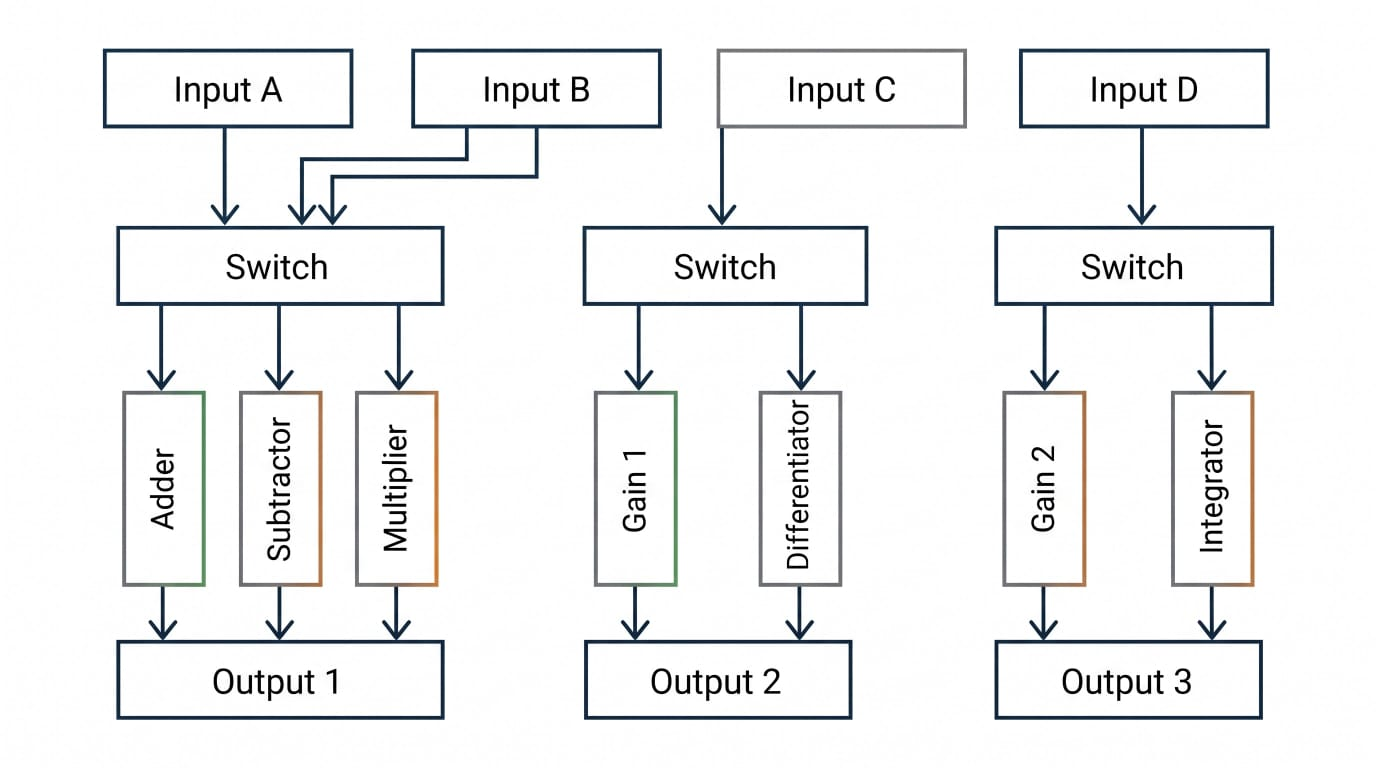
\includegraphics[width=0.62\textwidth]{images/BlockDiagram.jpeg}
    \caption{System Block Diagram}
    \label{fig:BlockDiagram}
\end{figure}
\section{Functional Organization and Signal Interfaces}
\subsection{Adder Circuit}


\begin{figure}[H]
    \centering
    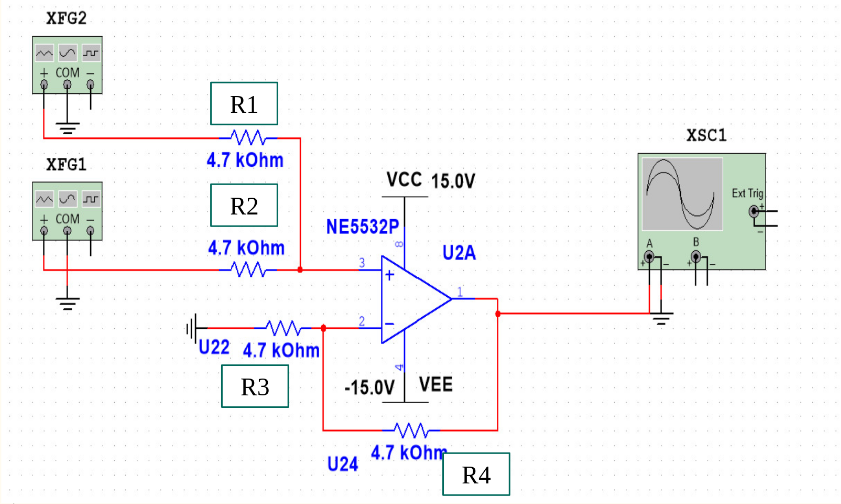
\includegraphics[width=0.6\textwidth]{images/Screenshot from 2026-11-17 14-42-07.png}
    \caption{Adder}
    \label{fig:Adder}
\end{figure}

\begin{equation}
\frac{v_1-v_+}{R_1}+\frac{v_2-v_+}{R_2}=0.
\end{equation}
Consequently,
\begin{equation}
v_+=\frac{R_2v_1+R_1v_2}{R_1+R_2}.
\end{equation}
The non-inverting closed-loop gain is $1+R_4/R_3$, so
\begin{equation}
v_{\mathrm{add}}=\left(1+\frac{R_4}{R_3}\right)
\frac{R_2v_1+R_1v_2}{R_1+R_2}.
\label{eq:addergeneral}
\end{equation}
With equal input resistors and $R_3=R_4$,
\begin{equation}
\boxed{v_{\mathrm{add}}=v_1+v_2.}
\label{eq:adder}
\end{equation}

\subsection{Subtractor Circuit}
\begin{figure}[H]
    \centering
    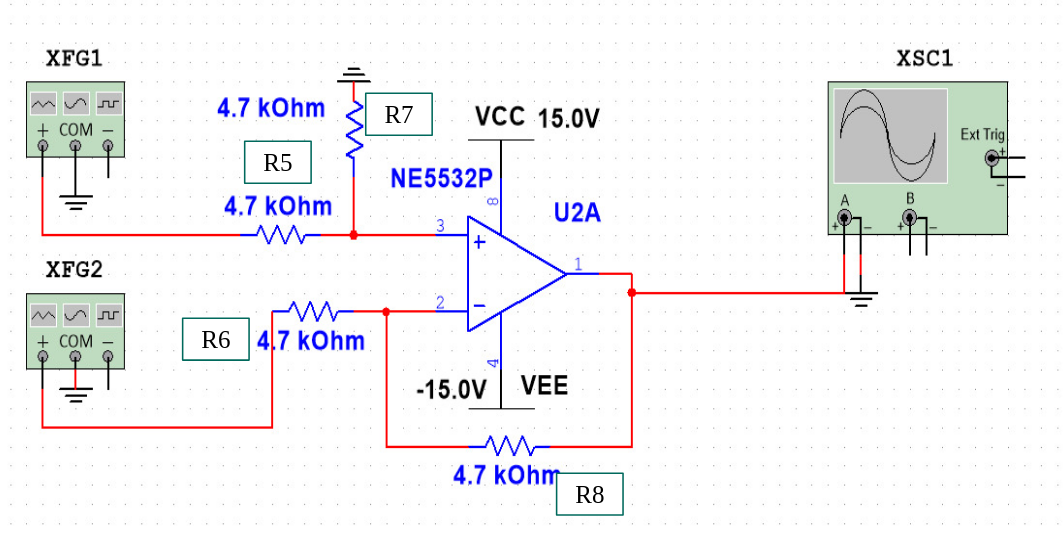
\includegraphics[width=0.55\textwidth]{images/Subtractor.png}
    \caption{Subtractor}
    \label{fig:Subtractor}
\end{figure}

The non-inverting input voltage is
\begin{equation}
v_+=\frac{R_7}{R_5+R_7}v_1.
\end{equation}
Using the virtual-short approximation under linear negative-feedback operation,
\begin{equation}
v_{\mathrm{sub}}=\left(1+\frac{R_8}{R_6}\right)
\frac{R_7}{R_5+R_7}v_1-\frac{R_8}{R_6}v_2.
\end{equation}
The balanced condition is $R_8/R_6=R_7/R_5=k$, giving
\begin{equation}
v_{\mathrm{sub}}=k(v_1-v_2).
\end{equation}
For the equal nominal values,
\begin{equation}
\boxed{v_{\mathrm{sub}}=v_1-v_2.}
\end{equation}


\subsection{Multiplier Circuit}
\subsubsection{Choice of Multiplication Method}
\begin{itemize}
    \item Two multiplication methods were considered: ring modulation and the Gilbert cell.
\item Ring modulation was found unsuitable for the project’s required 10 kHz operation, so a Gilbert-cell multiplier was selected.
\item The Gilbert cell consists of six transistors arranged as a lower differential pair and an upper transistor quad.
\item Through current steering, it produces a differential output proportional to the product of the two inputs when operated within its linear range.
    
\end{itemize}
\subsubsection{Input Scaling and Opposite-Polarity Signals}
\begin{figure}[H]
    \centering
    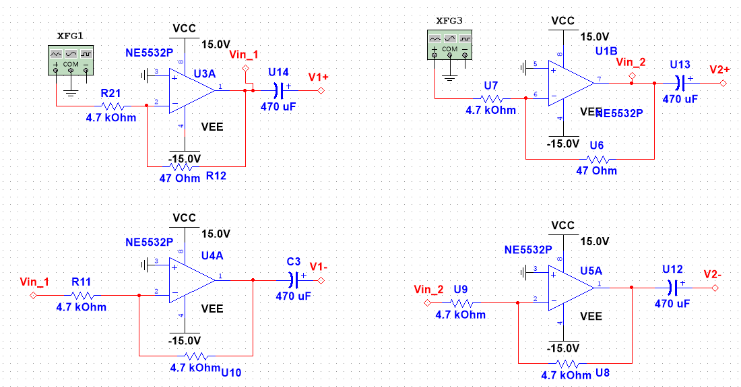
\includegraphics[width=0.7\textwidth]{images/input_scaler.png}
    \caption{Input Scaling}
    \label{fig:InputScaling}
\end{figure}

The first channel of IC2 uses R9~=~4.7~\kohm\ and R10~=~47~\ohm. Its nominal inverting gain is

\begin{equation}
A_{2A}=-\frac{R_{10}}{R_9}=-\frac{47}{4700}=-0.01.
\end{equation}


C1--C4 couple these conditioned signals into the biased transistor circuit.470~\uF\ coupling component~\cite{panasonic}. These capacitors separate the op-amp output DC level from the transistor bias level. 
For an illustrative effective bias resistance of 4.7~\kohm, the coupling corner is
\begin{equation}
f_c\approx\frac{1}{2\pi(4.7\times10^3)(470\times10^{-6})}
\approx0.072~\mathrm{Hz}.
\end{equation}

\subsubsection{Gilbert-Cell Operating Principle}
For an ideal matched BJT differential pair with tail current $I_T$, the difference in collector currents can be expressed as
\begin{equation}
i_d=I_T\tanh\left(\frac{v_d}{2V_T}\right),
\end{equation}
where $V_T=k_BT/q$ is the thermal voltage. An idealized Gilbert core consequently has the form
\begin{equation}
i_o\approx I_T\tanh\left(\frac{v_x}{2V_T}\right)
\tanh\left(\frac{v_y}{2V_T}\right).
\end{equation}
For internal differential voltages sufficiently small relative to $2V_T$,
\begin{equation}
i_o\approx\frac{I_T}{4V_T^2}v_xv_y.
\end{equation}
The collector resistors convert the differential currents into voltages. After differential recovery and adjustable gain, the intended system relation is
\begin{equation}
\boxed{v_{\mathrm{mul}}=K_m v_1v_2,}
\label{eq:multiplier}
\end{equation}

\begin{figure}[H]
    \centering
    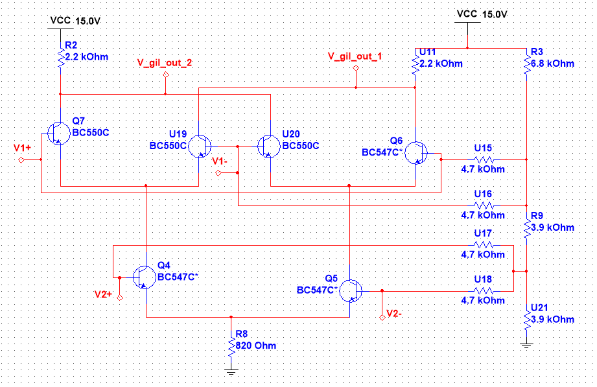
\includegraphics[width=0.7\textwidth]{images/gilbert.png}
    \caption{Gilbert Cell}
    \label{fig:GilbertCell}
\end{figure}

\subsubsection{Output Recovery}
\begin{figure}[H]
    \centering
    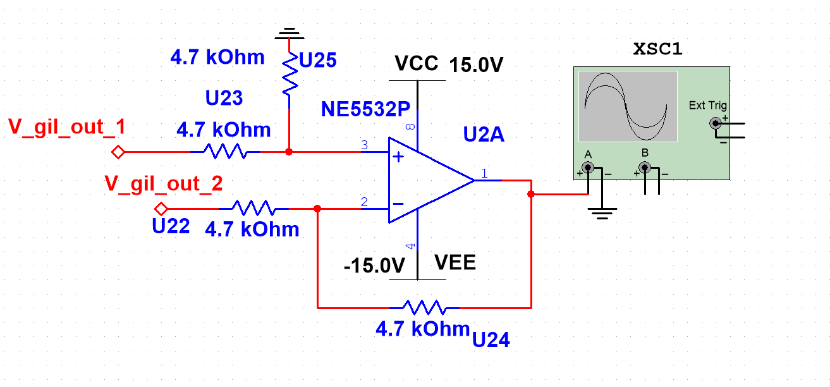
\includegraphics[width=0.7\textwidth]{images/subtr_mul.png}
    \caption{Subtractor for Multiplier}
    \label{fig:Subtractor_Multiplier}
\end{figure}

A subtractor circuit produces the difference between the two Gilbert-cell outputs:
\begin{equation}
v_{\mathrm{diff}} = v_{\mathrm{gill,out,1}} - v_{\mathrm{gill,out,2}}.
\end{equation}
A gain-control stage adjusts the multiplier scaling factor $K$, giving the final output:
\begin{equation}
v_{\mathrm{out}} = K v_1 v_2.
\end{equation}
\subsubsection{Expected Multiplication Tests and Limitations}
For two sinusoidal inputs,
\begin{align}
v_1(t)&=A\sin(2\pi f_1t),\\
v_2(t)&=B\sin(2\pi f_2t),
\end{align}
the ideal product is
\begin{equation}
v_{\mathrm{mul}}(t)=\frac{K_mAB}{2}
\left[\cos\bigl(2\pi(f_1-f_2)t\bigr)-\cos\bigl(2\pi(f_1+f_2)t\bigr)\right].
\end{equation}


\subsection{Differentiator Circuit}

The differentiator stage is an active inverting op-amp circuit that built around a NE5532P (U1A). A switched bank of input capacitors selects one of four operating bands, so the output stays within the op-amp's linear range across the full $1\,\text{Hz}$--$10\,\text{kHz}$ input range. Figure~\ref{fig:differentiator} shows the circuit as simulated.

\begin{figure}[H]
	\centering
	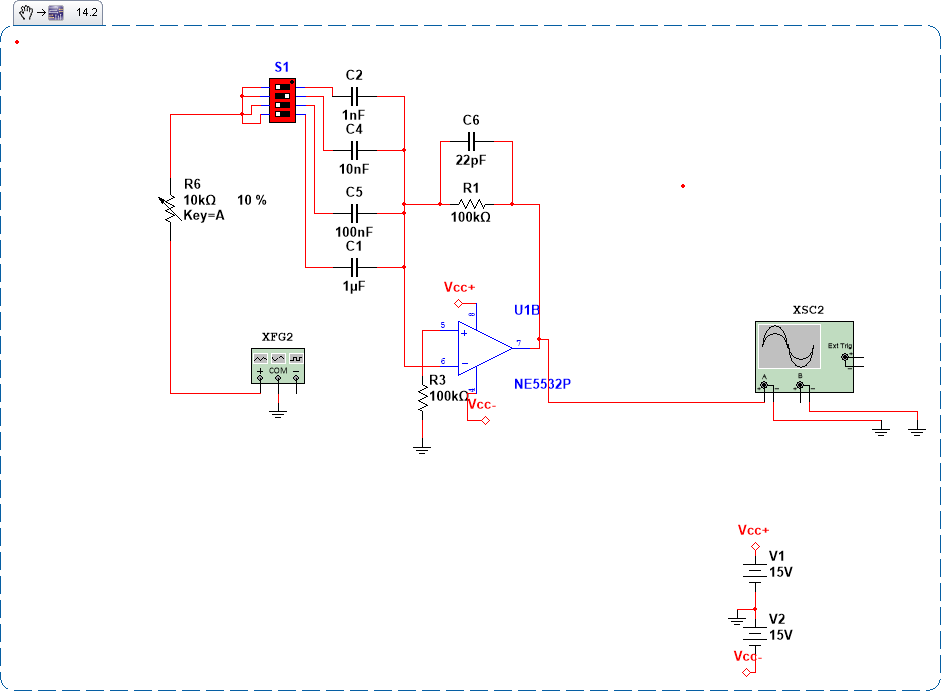
\includegraphics[width=0.75\textwidth]{images/differentiator_1.png}
	\caption{Active differentiator circuit simulation.}
	\label{fig:differentiator}
\end{figure}

\subsubsection{Transfer Function and Constant Derivation}

For a practical op-amp differentiator with input resistor $R_{in}$, input capacitor $C_{in}$, feedback resistor $R_f$ and parallel feedback capacitor $C_f$, the impedances are
\begin{equation}
	Z_{in}(s) = R_{in} + \frac{1}{sC_{in}} = \frac{1 + sR_{in}C_{in}}{sC_{in}},
\end{equation}
\begin{equation}
	Z_f(s) = R_f \parallel \frac{1}{sC_f} = \frac{R_f}{1 + sR_fC_f}.
\end{equation}
Using the inverting configuration gain $H(s) = -Z_f(s)/Z_{in}(s)$, the transfer function is
\begin{equation}
	H_{diff}(s) = -\frac{sR_fC_{in}}{(1 + sR_{in}C_{in})(1 + sR_fC_f)}.
	\label{eq:diff_tf}
\end{equation}

Within the operating band, where $f \ll \frac{1}{2\pi R_{in}C_{in}}$ and $f \ll \frac{1}{2\pi R_fC_f}$, both pole terms are approximately $1$ and Equation~\eqref{eq:diff_tf} reduces to
\begin{equation}
	H_{diff}(s) \approx -s\,(R_fC_{in}).
\end{equation}
Taking the inverse Laplace transform gives the time-domain relation
\begin{equation}
	v_{out}(t) = -K\,\frac{dv_{in}(t)}{dt}, \qquad K = R_fC_{in}\ [\text{s}],
	\label{eq:diff_time}
\end{equation}
where $K$ is the differentiation scaling constant. Since the output is DC-coupled, $H_{out}(s) = 1$ and the overall system transfer function equals $H_{diff}(s)$.

\subsubsection{Frequency Band Specifications}
\begin{itemize}
	\item \textbf{Operating range:} DC to $10\,\text{kHz}$.
	\item \textbf{Lower cutoff frequency ($f_L$):} $0\,\text{Hz}$ (DC-coupled output).
	\item \textbf{Upper cutoff frequency ($f_H$):} set by the feedback network ($R_1$, $C_6$):
\end{itemize}
\begin{equation}
	f_H = \frac{1}{2\pi R_1 C_6} = \frac{1}{2\pi\,(100\,\text{k}\Omega)(150\,\text{pF})} \approx 10.61\,\text{kHz} \approx 10\,\text{kHz}.
\end{equation}

\subsubsection{Switch-Wise Scaling Factors and Output Equations}

With $R_f = R_1 = 100\,\text{k}\Omega$, each switch position selects one capacitor and therefore one value of $K$, as listed in Table~\ref{tab:diff_scaling}.

\begin{table}[htbp]
	\centering
	\caption{Scaling factor $K = R_fC_{in}$ for each switch position.}
	\label{tab:diff_scaling}
	\begin{tabular}{|c|c|c|c|c|}
		\hline
		\textbf{Switch} & \textbf{Band} & $\bm{C_{in}}$ & \textbf{Calculation} & $\bm{K}$ \\
		\hline
		4 & $1$--$5\,\text{Hz}$ & $C_1 = 1\,\mu\text{F}$ & $100\,\text{k}\Omega \times 1\,\mu\text{F}$ & $0.1\,\text{s}$ \\ \hline
		3 & $5$--$10\,\text{Hz}$ & $C_5 = 100\,\text{nF}$ & $100\,\text{k}\Omega \times 100\,\text{nF}$ & $0.01\,\text{s}$ \\ \hline
		2 & $10\,\text{Hz}$--$1\,\text{kHz}$ & $C_4 = 10\,\text{nF}$ & $100\,\text{k}\Omega \times 10\,\text{nF}$ & $1\,\text{ms}$ \\ \hline
		1 & $1$--$10\,\text{kHz}$ & $C_2 = 1\,\text{nF}$ & $100\,\text{k}\Omega \times 1\,\text{nF}$ & $100\,\mu\text{s}$ \\ \hline
	\end{tabular}
\end{table}

\subsection{Integrator Circuit}
The integrator stage is an active inverting op-amp circuit built around an NE5532P (U1B). A switched bank of feedback capacitors selects one of four operating bands, so the output stays within the op-amp's linear range across the full $1\,\text{Hz}$--$10\,\text{kHz}$ input range. Figure~\ref{fig:integrator} shows the circuit as simulated.

\begin{figure}[H]
	\centering
	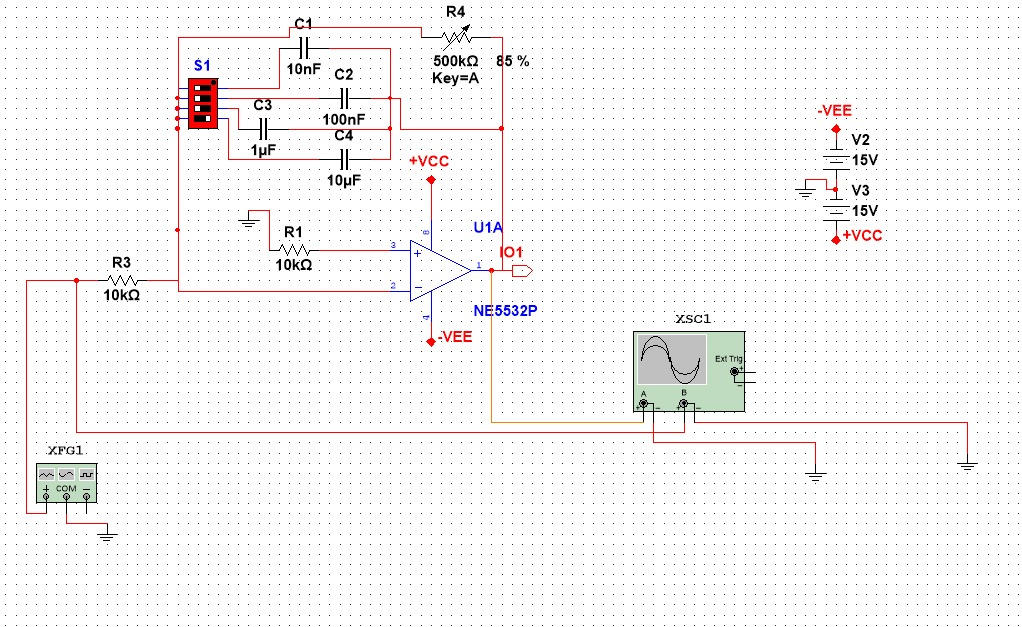
\includegraphics[width=0.75\textwidth]{images/Integrator.jpeg}
	\caption{Active integrator circuit simulation.}
	\label{fig:integrator}
\end{figure}

\subsubsection{Transfer Function and Constant Derivation}

For a practical active op-amp integrator with input resistor $R_{in}$, feedback capacitor $C_f$ and parallel feedback resistor $R_f$, the impedances are
\begin{equation}
	Z_{in}(s) = R_{in},
\end{equation}
\begin{equation}
	Z_f(s) = R_f \parallel \frac{1}{sC_f} = \frac{R_f}{1 + sR_fC_f}.
\end{equation}
Using the inverting configuration gain $H(s) = -Z_f(s)/Z_{in}(s)$, the transfer function is
\begin{equation}
	H_{int}(s) = -\frac{R_f}{R_{in}}\cdot\frac{1}{1 + sR_fC_f}.
	\label{eq:int_tf}
\end{equation}

Within the integration region, where $f \gg \frac{1}{2\pi R_fC_f}$, the denominator of Equation~\eqref{eq:int_tf} is approximated as $1 + sR_fC_f \approx sR_fC_f$, so the transfer function simplifies to
\begin{equation}
	H_{int}(s) \approx -\frac{1}{sR_{in}C_f}.
\end{equation}
Taking the inverse Laplace transform gives the time-domain relation
\begin{equation}
	v_{out}(t) = -\frac{1}{\tau}\int v_{in}(t)\,dt, \qquad \tau = R_{in}C_f\ [\text{s}],
	\label{eq:int_time}
\end{equation}
where $\tau$ is the integration time constant. Since the output is DC-coupled, there is no additional output filtering or coupling network, so $H_{out}(s) = 1$ and the overall system transfer function equals $H_{int}(s)$.

\subsubsection{Frequency Band Specifications}
\begin{itemize}
	\item \textbf{Operating range:} $1\,\text{Hz}$ to $10\,\text{kHz}$.
	\item \textbf{Lower cutoff frequency ($f_L$):} set by the feedback network ($R_4$, $C_f$). Integration is valid only for frequencies well above
\end{itemize}
\begin{equation}
	f_L = \frac{1}{2\pi R_4 C_f}.
\end{equation}
For example, with $R_4 = 500\,\text{k}\Omega$ and $C_f = C_4 = 10\,\mu\text{F}$, $f_L \approx 0.032\,\text{Hz}$.

\subsubsection{Switch-Wise Frequency Range Support}

With $R_{in} = R_3 = 10\,\text{k}\Omega$, each switch position selects one feedback capacitor and therefore one time constant $\tau$, as listed in Table~\ref{tab:int_scaling}.

\begin{table}[htbp]
	\centering
	\caption{Time constant $\tau = R_{in}C_f$ for each switch position.}
	\label{tab:int_scaling}
	\begin{tabular}{|c|c|c|c|c|}
		\hline
		\textbf{Switch} & \textbf{Band} & $\bm{C_f}$ & \textbf{Calculation} & $\bm{\tau}$ \\
		\hline
		4 & $1$--$10\,\text{Hz}$ & $C_4 = 10\,\mu\text{F}$ & $10\,\text{k}\Omega \times 10\,\mu\text{F}$ & $100\,\text{ms}$ \\ \hline
		3 & $10$--$100\,\text{Hz}$ & $C_3 = 1\,\mu\text{F}$ & $10\,\text{k}\Omega \times 1\,\mu\text{F}$ & $10\,\text{ms}$ \\ \hline
		2 & $100\,\text{Hz}$--$1\,\text{kHz}$ & $C_2 = 100\,\text{nF}$ & $10\,\text{k}\Omega \times 100\,\text{nF}$ & $1\,\text{ms}$ \\ \hline
		1 & $1$--$10\,\text{kHz}$ & $C_1 = 10\,\text{nF}$ & $10\,\text{k}\Omega \times 10\,\text{nF}$ & $0.1\,\text{ms}$ \\ \hline
	\end{tabular}
\end{table}



\subsection{Gain-Control}

\section{Component Selection}
\subsection{NE5532 Operational Amplifiers}

\noindent
\begin{minipage}[t]{0.62\textwidth}
    \vspace{0pt}
    \begin{itemize}
        
		\item Typical specifications are a 12~MHz unity-gain bandwidth,
        a 5~V/$\mu$s slew rate, and an input voltage noise of
        5~nV/$\sqrt{\mathrm{Hz}}$ at 1~kHz.

        \item A 10~kHz sine wave with a 10~V peak output requires a slew
        rate of 0.628~V/$\mu$s, below the typical device rating.
    \end{itemize}
\end{minipage}\hfill%
\begin{minipage}[t]{0.34\textwidth}
    \vspace{0pt}
    \centering
    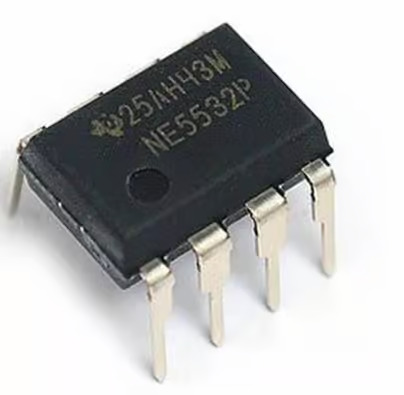
\includegraphics[width=0.5\linewidth]{images/ne5532.jpg}
    \captionof{figure}{NE5532D dual operational amplifier.}
    \label{fig:ne5532}
\end{minipage}


\subsection{BC550C Transistors}
\noindent
\begin{minipage}[t]{0.62\textwidth}
    \vspace{0pt}
    \begin{itemize}
        \item The Gilbert-cell multiplier uses six low-noise BC550C NPN
        transistors (Q1--Q6).

        \item The maximum collector-emitter voltage is 45~V and the
        maximum DC collector current is 100~mA. The DC current gain
        $h_{FE}$ ranges from 420 to 800 under the datasheet test
        conditions~\cite{bc550}.

        \item Matching the transistors and keeping them at similar
        temperatures improves multiplier balance.
    \end{itemize}
\end{minipage}\hfill%
\begin{minipage}[t]{0.34\textwidth}
    \vspace{0pt}
    \centering
    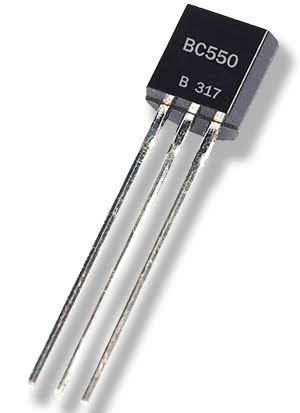
\includegraphics[width=0.5\linewidth]{images/BC550.jpeg}
    \captionof{figure}{BC550C NPN transistor.}
    \label{fig:bc550c}
\end{minipage}

\subsection{Resistors, Capacitors, and Controls}
    \begin{itemize}
        \item The Gilbert cell requires closely matched collector resistors ($R_C$)
	in its differential stages. We ordered resistors with a 0.1\% tolerance
	and selected SMD packages to keep connections short and reduce noise pickup.

		\item We selected SMD capacitors to save PCB space and reduce noise pickup
b		y keeping connecting traces short.
    \end{itemize}


\section{PCB Design}
\begin{minipage}[t]{0.5\textwidth}
    \vspace{0pt}
    \centering
    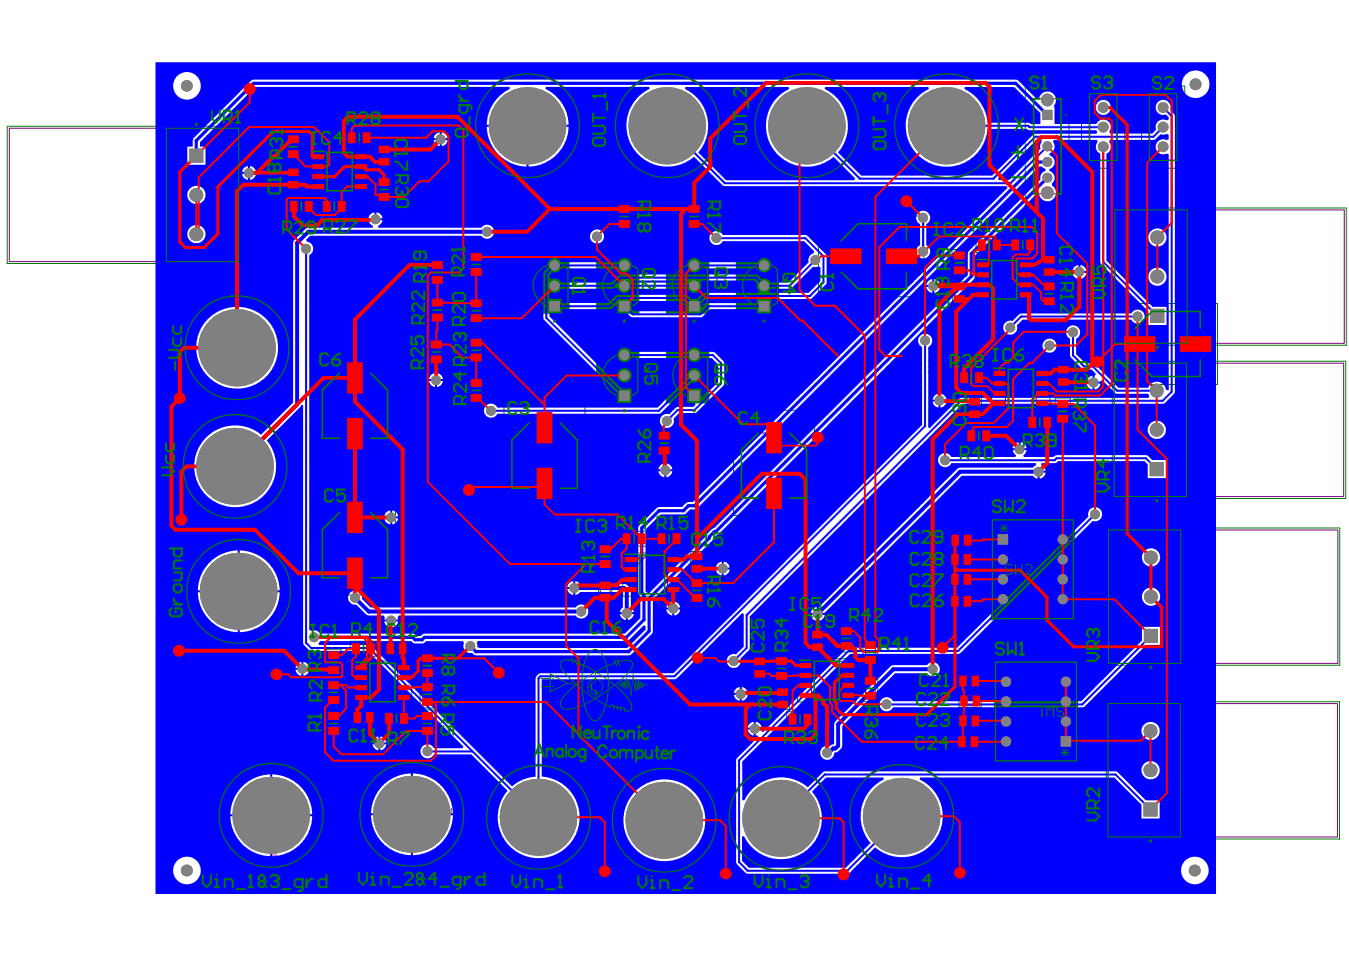
\includegraphics[width=\linewidth]{images/PCB.png}
    \captionof{figure}{PCB layout }
    \label{fig:pcb}
\end{minipage}\hfill%
\begin{minipage}[t]{0.5\textwidth}
    \vspace{0pt}
    \centering
    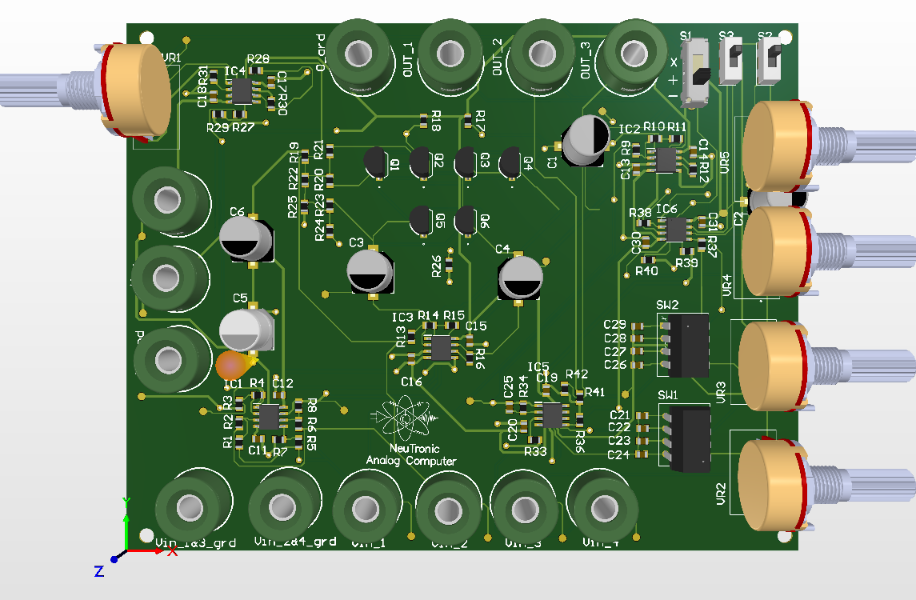
\includegraphics[width=\linewidth]{images/PCB_3D.png}
    \captionof{figure}{3D PCB layout}
    \label{fig:pcb}
\end{minipage}

The circuit is implemented on a two-layer PCB, with signal traces routed on the top layer and a ground plane on the bottom layer.

The PCB provides three output ports, each controlled independently by a dedicated selector switch. The first switch routes the output of the adder, subtractor, or multiplier to the first port. The second switch selects between the differentiator and the first gain stage, while the third switch selects between the integrator and the second gain stage.

Input signals are supplied through four banana jacks. Two jacks provide the common pair of inputs to the adder, subtractor, and multiplier. A third jack supplies the differentiator and the first gain stage, while a fourth jack supplies the integrator and the second gain stage.

\section{Enclosure Design}

\begin{minipage}[t]{0.48\textwidth}
    \vspace{0pt}
    \centering
    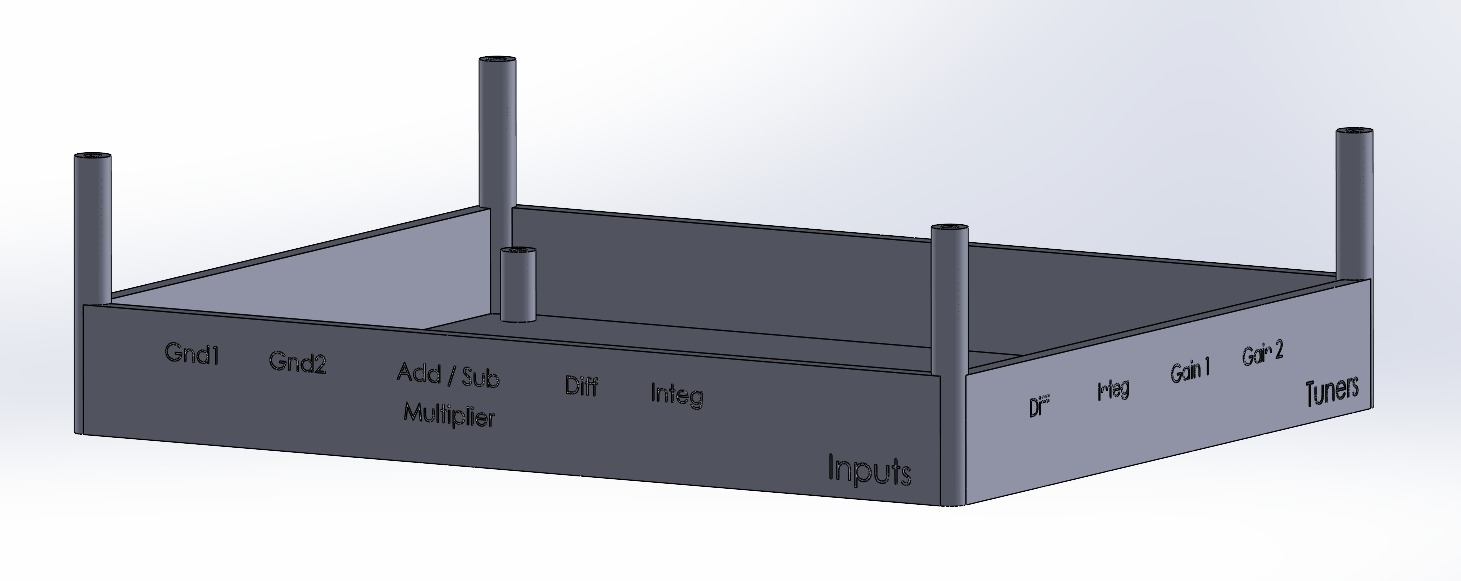
\includegraphics[width=0.8\linewidth]{images/Enclosure_Below.jpeg}
    \captionof{figure}{Enclosure bottom view}
    \label{fig:Enclosure_Below}
\end{minipage}\hfill%
\begin{minipage}[t]{0.48\textwidth}
    \vspace{0pt}
    \centering
    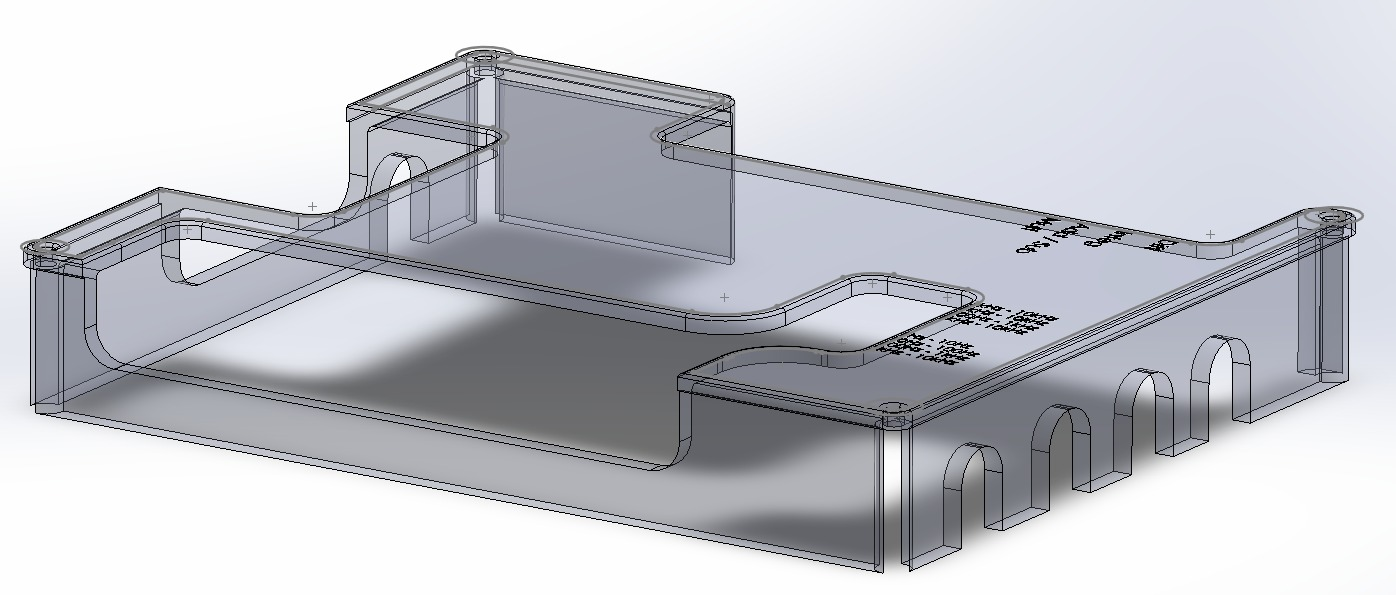
\includegraphics[width=0.8\linewidth]{images/Enclosure_top.jpeg}
    \captionof{figure}{Enclosure top view}
    \label{fig:Enclosure_Top}
\end{minipage}
\begin{figure}[H]
    \centering
    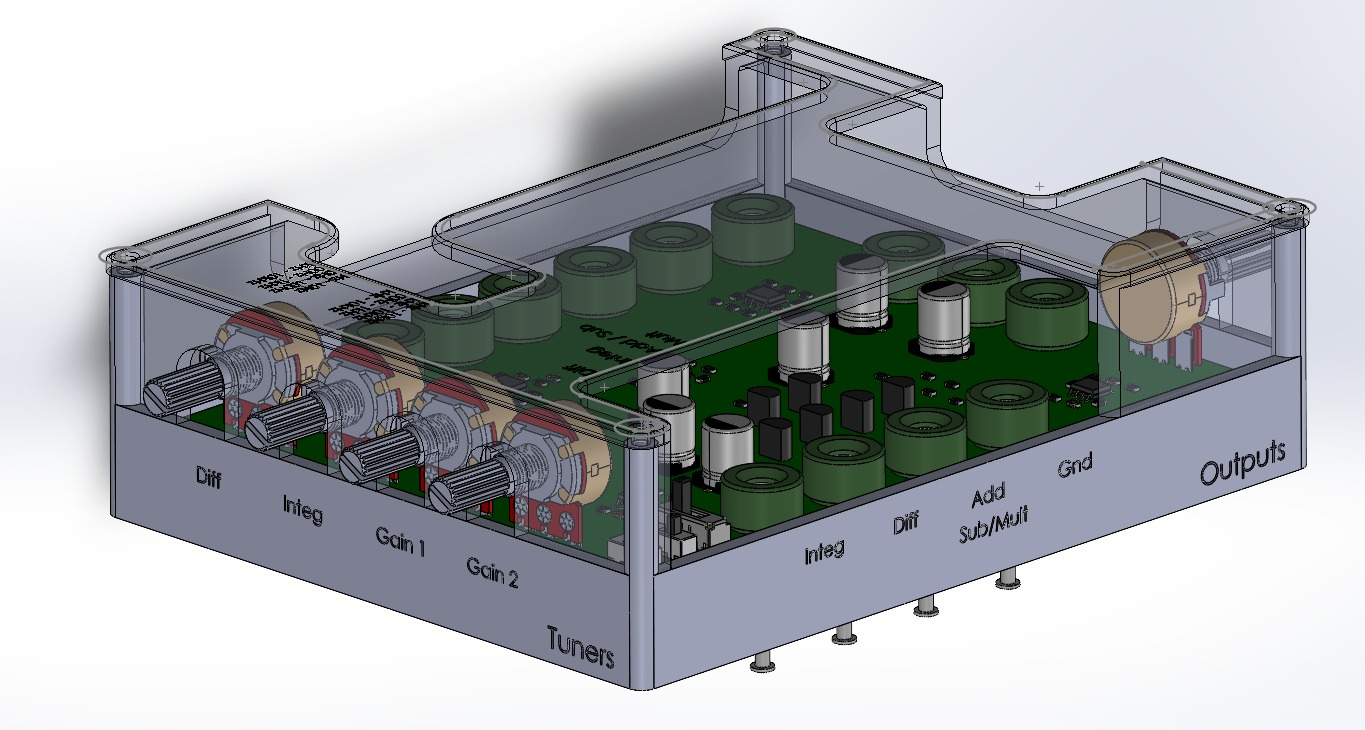
\includegraphics[width=0.4\textwidth]{images/Final.jpeg}
    \caption{Final PCB Implementation}
    \label{fig:FinalPCB}
\end{figure}
\section{Software Simulation and Hardware Testing}
\subsection{Software Simulation}
\begin{minipage}[t]{0.48\textwidth}
    \vspace{0pt}
    \centering
    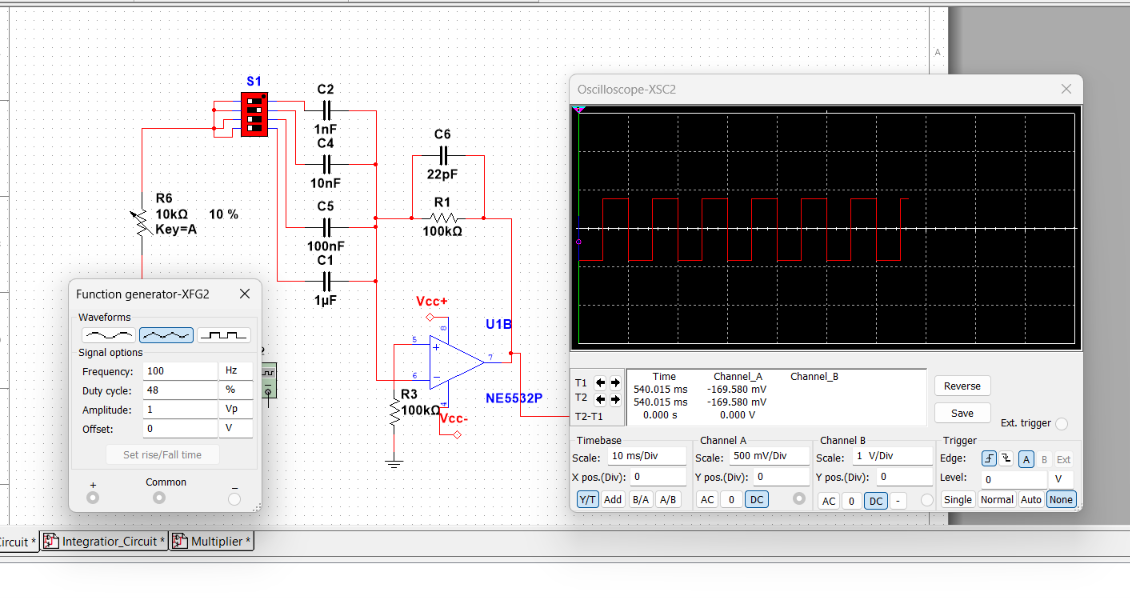
\includegraphics[width=\linewidth]{images/Diiferentiator_Sim.png}
    \captionof{figure}{Differentiator simulation}
    \label{fig:DiffSim}
\end{minipage}\hfill%
\begin{minipage}[t]{0.48\textwidth}
    \vspace{0pt}
    \centering
    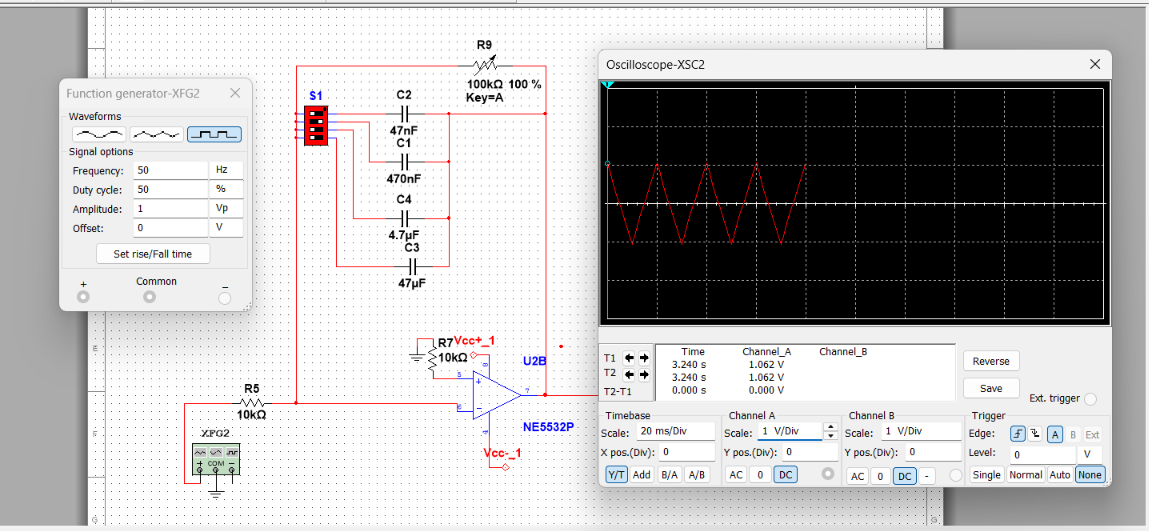
\includegraphics[width=\linewidth]{images/Integ sim.png}
    \captionof{figure}{Integrator Simulation}
    \label{fig:IntSim}
\end{minipage}
\begin{minipage}[t]{0.48\textwidth}
    \vspace{0pt}
    \centering
    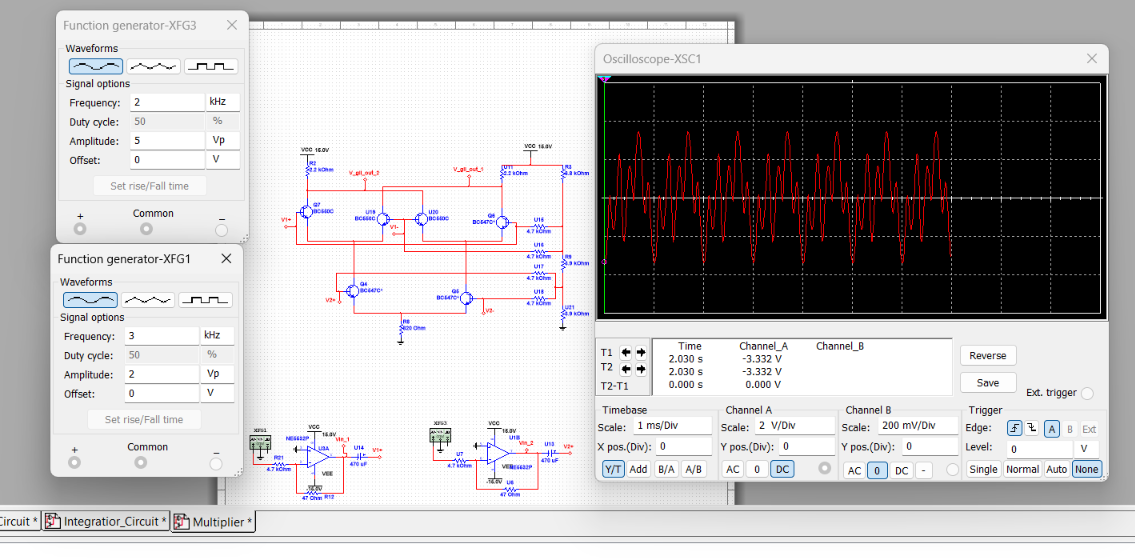
\includegraphics[width=\linewidth]{images/Multiplier_Sim.png}
    \captionof{figure}{Multiplier Simulation}
    \label{fig:MultSim}
\end{minipage}\hfill%

The simulation stage used Multisim to verify the circuit design and expected behaviour. The differentiator, integrator, and multiplier circuits were simulated with representative input signals, and the output waveforms were compared to theoretical expectations. The simulations confirmed that the circuits operated correctly within the specified frequency range and provided the expected mathematical operations on the input signals.


\subsection{Breadboard Implementation and Testing}

\begin{minipage}[t]{0.45\textwidth}
    \vspace{0pt}
    \centering
    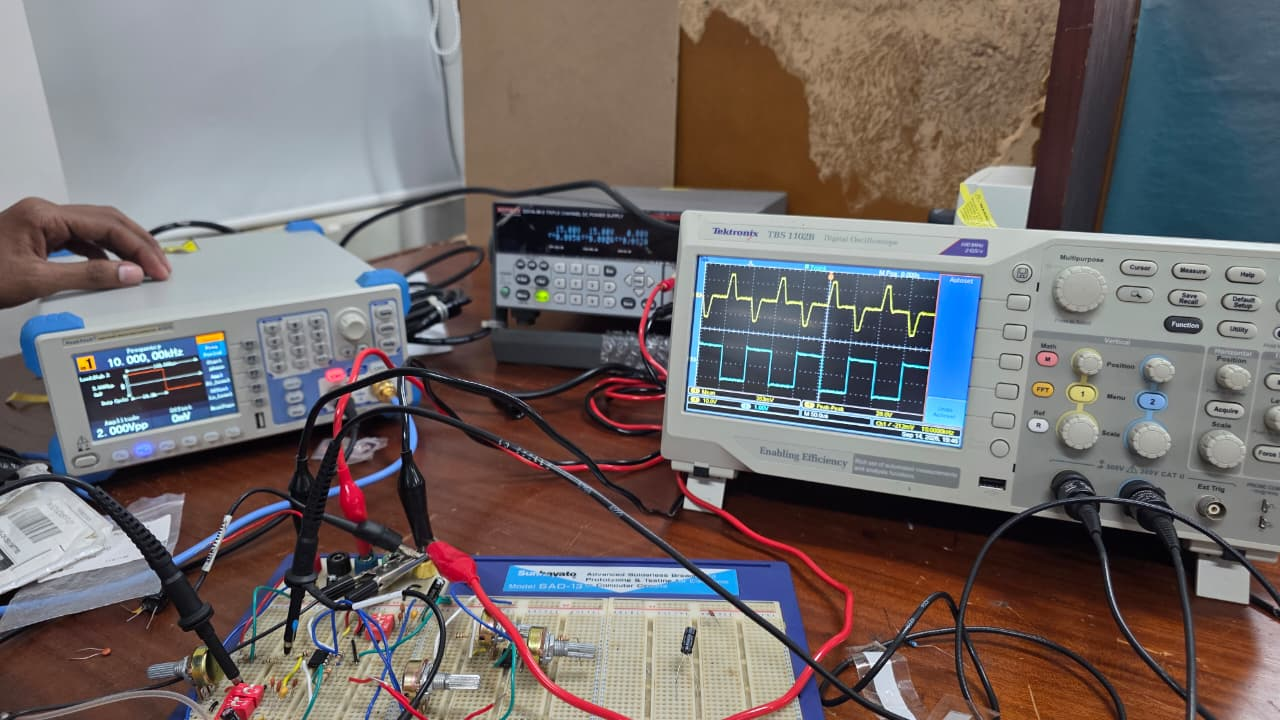
\includegraphics[width=\linewidth]{images/differentiator.jpeg}
    \captionof{figure}{Differentiator circuit}
    \label{fig:differentiator}
\end{minipage}\hfill%
\begin{minipage}[t]{0.45\textwidth}
    \vspace{0pt}
    \centering
    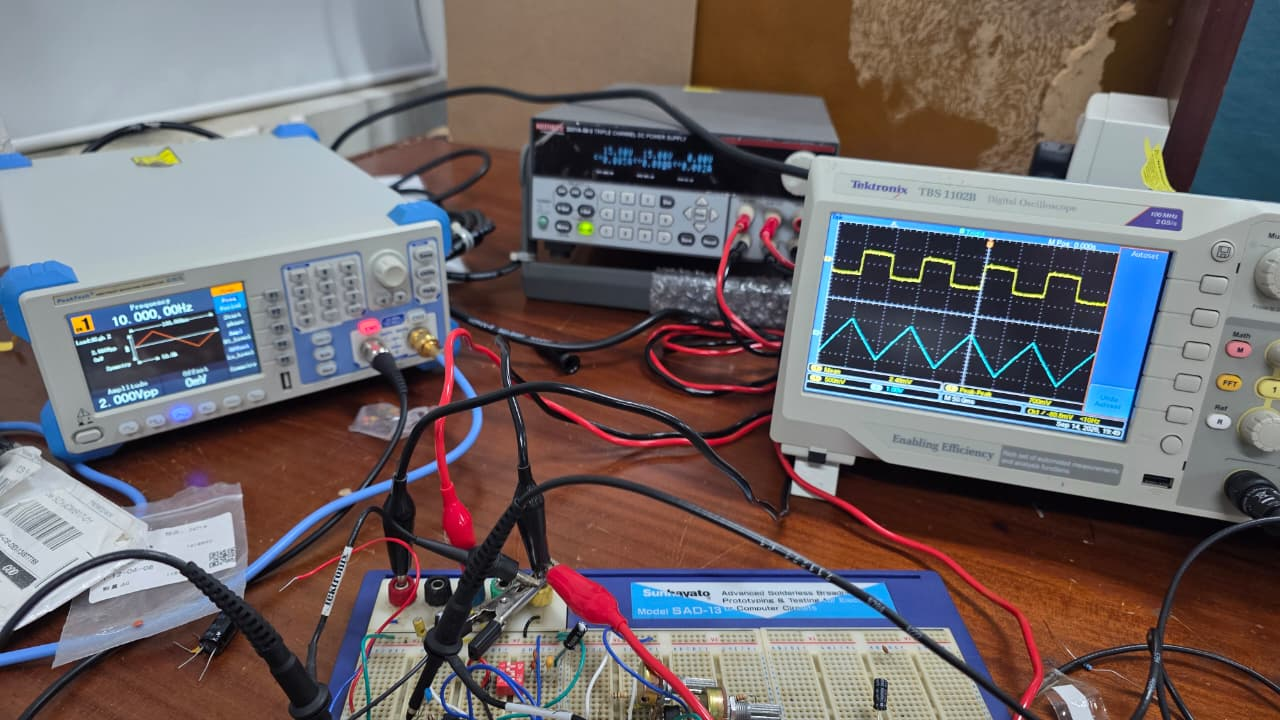
\includegraphics[width=\linewidth]{images/B_int.jpeg}
    \captionof{figure}{Integrator circuit}
    \label{fig:integrator}
\end{minipage}
\begin{figure}[H]
    \centering
    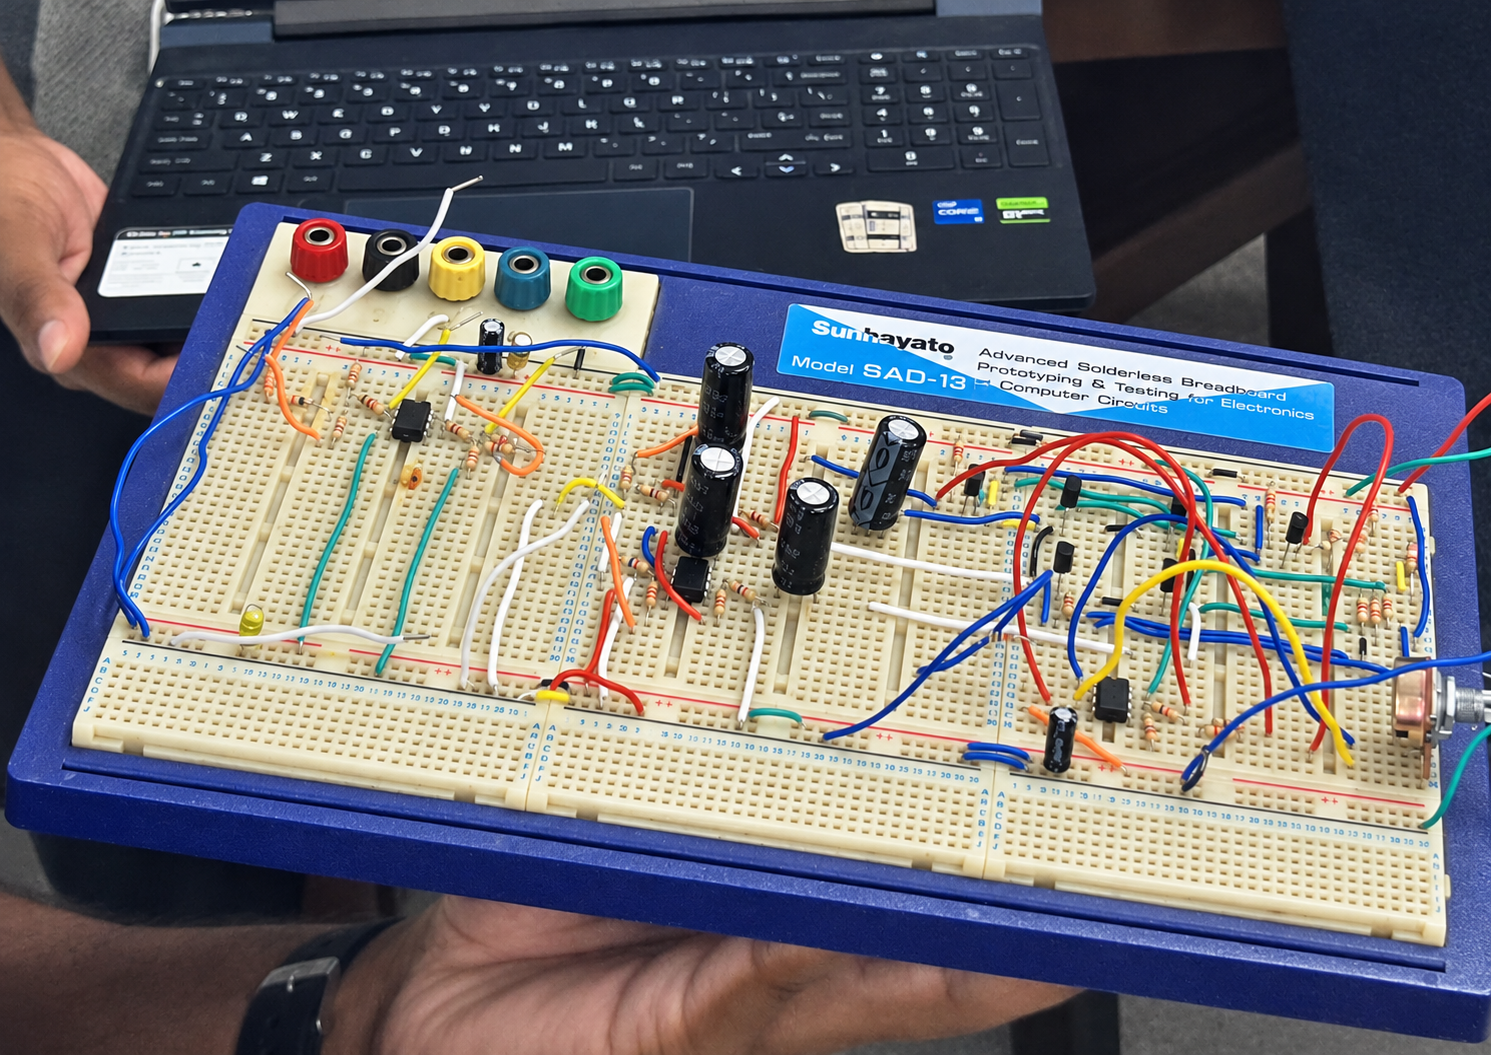
\includegraphics[width=0.45\textwidth]{images/Breadboard.png}
    \caption{Adder,Subtractor, and Multiplier breadboard prototype.}
    \label{fig:BreadBoard Prototype}
\end{figure}



We constructed and tested breadboard prototypes after simulation. This stage provided the opportunity to inspect practical polarity, biasing, gain, clipping, and waveform behaviour before committing to the PCB.

Breadboards introduce long connection loops, contact uncertainty, and parasitic capacitance. These effects are especially relevant to the differentiator and discrete multiplier. Short feedback paths, local bypassing, consistent grounding, and suitable signal amplitudes help separate circuit behaviour from the test setup.

\subsection{Final PCB Implementation}

\begin{minipage}[t]{0.45\textwidth}
    \vspace{0pt}
    \centering
    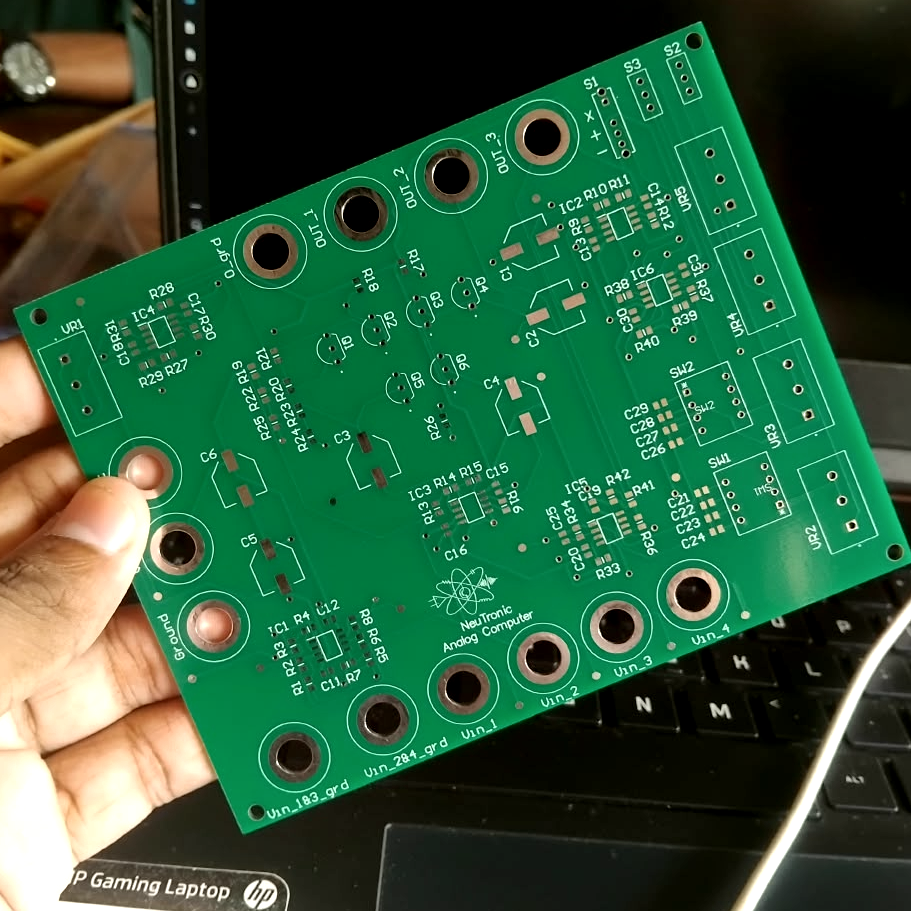
\includegraphics[width=0.8\textwidth]{images/PCB_Before.png}
    \captionof{figure}{Final PCB Before Soldering}
    \label{fig:PCB_Before}
\end{minipage}\hfill%
\begin{minipage}[t]{0.45\textwidth}
    \vspace{0pt}
    \centering
    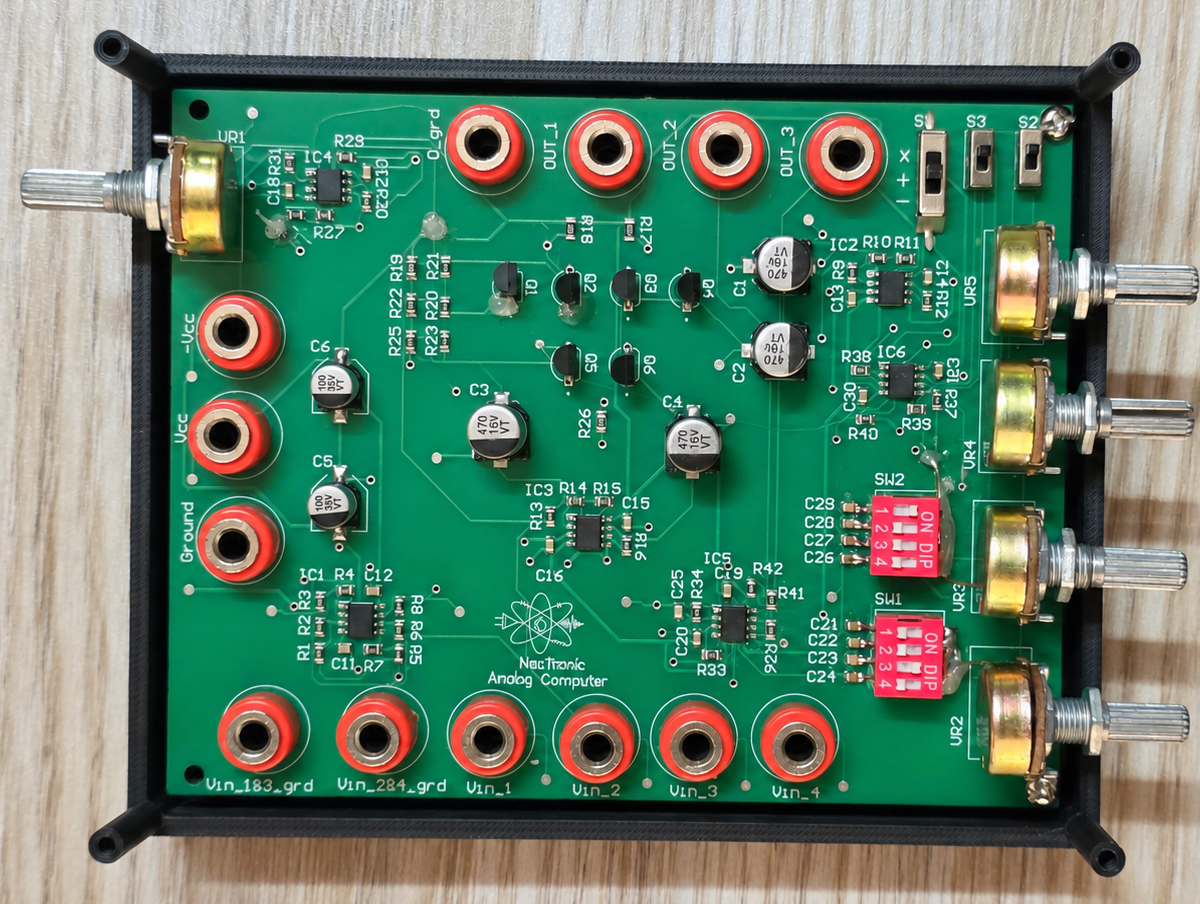
\includegraphics[width=\textwidth]{images/after.png}
    \captionof{figure}{Final PCB After Soldering}
    \label{fig:PCB_After}
\end{minipage}


\subsection{Discussion of Accuracy and Practical Limitations}

\begin{itemize}
    \item \textbf{Circuit accuracy and breadboard testing.} Component tolerances affected accuracy, and breadboard tests with through-hole resistors showed noisy, unstable outputs.

    \item \textbf{Multiplier transistor matching.} A local BC550 shortage made it difficult to match six transistor pairs for $h_{\mathrm{FE}}$. Mismatch contributed to carrier leakage and extended debugging.

    \item \textbf{PCB fabrication and assembly.} A temporary manufacturer closure delayed fabrication. A switch footprint issue left 16 pins across two switches shorted to the ground plane. Jumper wires beneath the PCB bypassed the affected connections.

    \item \textbf{Performance verification.} Measuring all five operations across the intended frequency and amplitude ranges is needed to quantify final PCB accuracy.
\end{itemize}

\section{Conclusion \& Future Works}
\subsection{Conclusion}
The project developed an analog computing platform around op-amp arithmetic stages, a discrete transistor multiplication core, switched calculus networks, adjustable controls. The work progressed from circuit analysis and software simulation to breadboard testing and final PCB implementation, with an accompanying enclosure design.The main outcome is practical understanding of how mathematical circuit models are affected by real devices, biasing, loading, tolerances, and layout.
\subsection{Future Improvements}
\begin{enumerate}
\item \textbf{Complete calibration and measurement.} Record amplitude, phase, frequency, DC offset, and load for every operation and range; establish a multiplier scale factor and usable input limits.
\item \textbf{Improve multiplier balance.} Select matched transistor pairs, improve thermal symmetry, evaluate a more stable bias arrangement, and provide repeatable offset and scale adjustment within the permitted component rules.
\item \textbf{Improve calculus controls.} Use clearly labelled range settings, consider mutually exclusive capacitor selection, and add an integrator reset or initialization control.
\item \textbf{Refine impedance and gain handling.} Evaluate dedicated input buffering and, if required, a true post-calculus gain stage. Such changes should be documented as revisions rather than attributed to the present selector topology.
\end{enumerate}

\section{Contribution of Group Members}
The work covered theoretical design, simulation, breadboard testing, PCB development, component assembly, enclosure design, and documentation.
% TODO: replace each contribution entry with the member's actual work.
% Do not copy the senior group's contribution assignments.
\begin{table}[htbp]
\centering\small
\caption{Project members and contribution record.}
\begin{tabularx}{\textwidth}{llY}
\toprule
\textbf{Index number} & \textbf{Name} & \textbf{Individual contribution}\\
\midrule
240445H & N. Naagul & Multiplier Circuit Design, PCB , Documentation.\\
240601J & P. Sathjaharan & Adder,Subtractor Circuit Design, PCB , Documentation.\\
240602M & B. Sathursan & Integrator Circuit Design, Enclosure , Documentation.\\
240525E & R. Prasannah & Differentiator Circuit Design, Enclosure , Documentation.\\
\bottomrule
\end{tabularx}
\end{table}

\section*{Acknowledgment}
\addcontentsline{toc}{section}{Acknowledgment}
We thank the academic staff and laboratory staff of the Department of Electronic and Telecommunication Engineering, University of Moratuwa, for the guidance and facilities associated with the EN~2091 Laboratory Practice and Projects module. We also acknowledge the contributions of all group members throughout the design, simulation, testing, and implementation stages. The earlier student report provided to the group was useful as a reference for the organization and presentation of the project documentation.
% TODO: add the correct supervisor/lecturer names only after confirming them.



\end{document}
